\documentclass{article}

% Language setting
% Replace `english' with e.g. `spanish' to change the document language
\usepackage[portuguese]{babel}

% Set page size and margins
% Replace `letterpaper' with`a4paper' for UK/EU standard size
\usepackage[a4paper,top=2cm,bottom=2cm,left=3cm,right=3cm,marginparwidth=1.75cm]{geometry}

% Useful packages
\usepackage{amsmath}
\usepackage{graphicx}
\usepackage[colorlinks=true, allcolors=blue]{hyperref}
\usepackage{float}
\usepackage{algorithm}
\usepackage{algpseudocode}

\graphicspath{{images/}}

\title{Lista de exercícios 4 \\
\large Árvore B}
\author{Lucas Emanuel Resck Domingues \\ \\
Estruturas de Dados e Algoritmos \\
Professor: Jean Roberto Ponciano}

\begin{document}

    \maketitle

    \begin{enumerate}
        \item Explique como encontrar a maior chave armazenada em uma árvore B.
        
        \bigskip
        
        \noindent \textbf{Solução:}


        \bigskip

        \item[3.] Escreva um algoritmo que, dada uma árvore B e uma chave, retorne o sucessor imediato da chave.
        
        \bigskip
        
        \noindent \textbf{Exercício 3} (2.5 pontos) Considerando o problema da mochila apresentado
previamente. Vamos supor que ao invés de somente um valor de prêmio
$v_i$ para cada item da mochila, existam $m$ valores de prêmio, e com isso
teremos múltiplos objetivos. Desenhe uma busca $A^\ast$ ou branch-and-bound
para esse problema.

\bigskip

\noindent \textbf{Solução:} 

% Comecemos com uma mochila uni-objetivo, por enquanto. Suponhamos que, em um esquema de árvore, computemos todas as possibilidades de mochila na força bruta. Isso é, a ramificação à esquerda do primeiro nó deixa o item 1 de fora, enquanto a ramificação à direita do primeiro nó considera o item 1 na mochila. E assim por diante, para cada item, realizando assim o \textit{branch}.

% Quando se atinge a capacidade máxima da mochila, não precisamos mais continuar seguindo no caminho daquele nó, pois, a cada novo item, ou ele não adiciona nenhum peso, ou ele adiciona algum peso, então toda a subárvore é não viável. Esse é o nosso \textit{bound}.

% Na verdade, podemos tomar uma estratégia mais interessante ainda: podemos utilizar algum outro algoritmo para checar o maior valor que será possível naquela subárvore. Podemos utilizar, por exemplo, uma relaxação do problema da mochila para um problema da mochila ``contínua'', que pode ser resolvida pelo algoritmo de \href{https://en.wikipedia.org/wiki/Continuous_knapsack_problem}{Dantzig}.\href{https://en.wikipedia.org/wiki/Continuous_knapsack_problem}{Dantzig}. De forma bem simples, o algoritmo enche a mochila utilizando quantidades fracionárias dos itens, colocando primeiro na mochila os itens mais ``valiosos'', então ele é tratável. Enquanto buscamos na árvore, mantemos um limitante inferior para o valor da mochila. Nós que possuem o melhor valor pela mochila contínua menor do que o limitante inferior são descartados, afinal, naquela subárvore, não seria possível obter uma solução melhor do que a solução da mochila contínua.

Inicialmente, vamos tratar da mochila uniobjetivo, para, posteriormente, generalizar o resultado para a mochila multiobjetivo. Para o problema da mochila original (uniobjetivo), podemos encontrar uma solução relaxada utilizando o algoritmo de \href{https://en.wikipedia.org/wiki/Continuous_knapsack_problem}{Dantzig}: um algoritmo guloso que enche a mochila com frações dos itens mais valiosos, ordenados pelo seu custo-benefício (valor dividido por peso), até que a mochila esteja cheia. Caso a solução resultante seja inteira, está tudo certo, e essa é a solução final.

Caso a solução para os itens não seja inteira (mais especificamente, as quantidades dos itens estejam entre $0$ e $w_i$), precisaremos ramificar. Ramificamos no item $i$ que possui o valor fracionário mais próximo de $0.5w_i$, e iniciamos na ramificação $0$ ou $w_i$, dependendo de o valor relaxado estar mais próximo de  $0$ ou $w_i$. Isso descreve completamente a sequência de $branches$.

Toda vez que calculamos um novo nó após uma ramificação, também encontramos o valor da mochila uniobjetivo dessa configuração relaxada. Isso significa que, naquela subárvore, todas as soluções, inteiras ou não, têm, no máximo, esse mesmo valor. Podemos armazenar uma variável chamada \textit{limitante inferior} de tal forma que, quando nos deparamos com uma subárvore que tem solução ótima contínua menor do que o limitante inferior, não chegamos nem a explorar as ramificações dessa árvore. Em outras palavras, só buscamos soluções melhores do que já temos.

O algoritmo descrito acima possui forte analogia com o branch-and-bound para problemas de programação linear, pelo menos no caso uni-objetivo.

Podemos generalizar esse algoritmo para o caso multiobjetivo da mochila. A princípio, o algoritmo permanece o mesmo para o \textit{branch} nas variáveis não inteirass. Porém, agora, vamos tomar outra estratégia para o \textit{bound}: vamos manter as soluções multiobjetivo armazenadas em uma lista chamada \textit{soluções não dominadas}, e só não vamos explorar uma subárvore quando (sua solução ótima contínua) for dominada por alguma das soluções já armazenadas. Se a solução ótima da mochila continua de um nó é dominada por alguma outra solução já armazenada, isso significa que todas as ramificações dentro dessa subárvore também o serão, afinal, os valores da mochila serão menores ou, no máximo, iguais aos valores ótimos da mochila contínua. Isso nos garante que, ao final do algoritmo, teremos apenas as \textbf{soluções não dominadas}, pois todas as dominadas foram descartadas.


        \bigskip

        \item[4.] Mostre, a cada passo, as árvores que resultam depois da remoção das chaves A, B,
        M, Q e R da árvore B de ordem 5 a seguir.

        \begin{figure}[H]
            \centering
            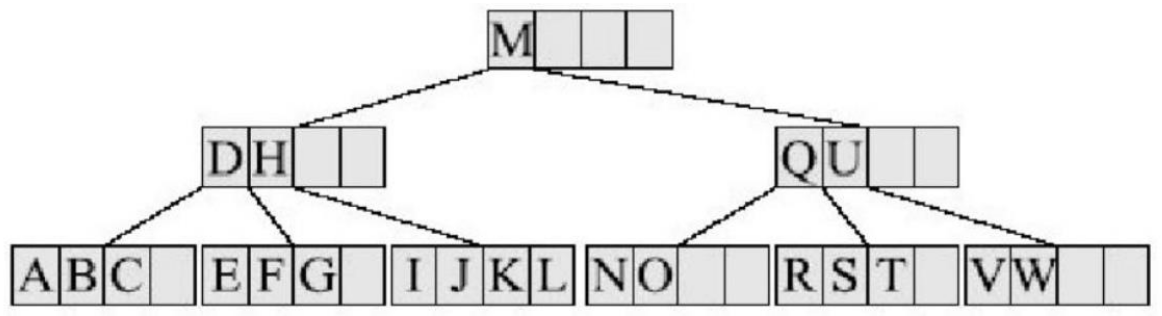
\includegraphics[width=0.6\linewidth]{tree.png}
        \end{figure}
        
        \bigskip
        
        \noindent \textbf{Exercício 4} (3.0 pontos) Suponha que temos $n$ tarefas onde cada uma toma
um tempo $t_i$ para processar em $m$ máquinas idênticas nas quais desejamos
dizer qual a sequência de tarefas em cada máquina. Uma mesma tarefa
não pode ser divida entre máquinas. Para um dado planejamento,
$A_j$ é o conjunto de tarefas colocados na máquina $j$.
Seja $L_j = \sum_{i \in A_j} t_i$ o tempo da
máquina $j$. O tempo de execução dessas tarefas será o maior $L_j$ dentre as
máquinas.
Nós consideramos um algoritmo guloso para esse problema que ordena
as tarefas de tal forma que $t_1 \ge t_2 \ge \cdots \ge t_n$ e iterativamente aloca o
próximo serviço na maquina com a menor carga.
Demonstre quão boa é a aproximação deste algoritmo (considerando OPT
é a solução ótima, esperamos algo menor que 2OPT).

\bigskip

\noindent \textbf{Solução:}


        \bigskip
    \end{enumerate}

\end{document}